\documentclass[12pt]{article}
\usepackage[utf8]{inputenc}
\usepackage[T2A]{fontenc}
\usepackage[russian]{babel}
\usepackage{amsmath}
\usepackage{amssymb}
\usepackage{dsfont}
\usepackage[dvipsnames]{xcolor}
\usepackage{setspace}
\usepackage{multirow}
\usepackage[a4paper, outer=1.5cm, inner=1.5cm, top=1cm, bottom=1cm]{geometry}
\usepackage{graphicx}
\usepackage{skull}
\usepackage{wasysym}
\usepackage{float}
\graphicspath{{.images/}}
\usepackage{hyperref}
\hypersetup{colorlinks=true, linkcolor=blue, filecolor=magenta, urlcolor=cyan}
\usepackage[firstpage]{draftwatermark}
\SetWatermarkText{
    $\qquad\qquad\qquad\qquad\qquad$\parbox{7cm}{\begin{center}
    
\includegraphics[width = 0.08\textwidth]{lion-logo.png}\bigskip\\~\bigskip\\~\vspace{-24mm}\\~\end{center}}
}
\SetWatermarkAngle{0}
\SetWatermarkScale{1.5}
\usepackage{etoolbox}

\newtoggle{ifsolved}
\newtoggle{needhelp}
\newcounter{num}
\setcounter{num}{1}

\newcommand{\newnum}{\par\textbf{\textnumero\arabic{num}}\stepcounter{num}}
\newcommand{\sol}{\vspace{3mm}\par\textbf{Решение: }}
\newcommand{\ans}{\vspace{3mm}\par\textbf{Ответ: }}
\newcommand{\hint}{\vspace{3mm}\par\textbf{Подсказка: }}
\newcommand{\mode}[1]{
\ifstrequal{#1}{0}{\togglefalse{ifsolved}\togglefalse{needhelp}}{\ifstrequal{#1}{1}{\togglefalse{ifsolved}\toggletrue{needhelp}}{\ifstrequal{#1}{2}{\toggletrue{ifsolved}\togglefalse{needhelp}}{\toggletrue{ifsolved}\toggletrue{needhelp}}}}} %if 0 - if 1 - if 2 - else
%\newenvironment{problem}[8]{%#1, #2, #3
%\parbox{\linewidth}{\vspace{4mm}\ifstrequal{#4}{(лёгкая)}{\newnum\textbf{.}}{\newnum\textbf{*.} } \\ #5}
%\iftoggle{ifsolved}{\sol #6}{}
%\iftoggle{ifsolved}{\ans #7}{}
%\iftoggle{needhelp}{\hint #8}{}}

\newenvironment{problem}[8]{%#1, #2, #3
\parbox{\linewidth}{\vspace{5mm}\ifstrequal{#4}{(лёгкая)}{\newnum\textbf{.}}{\newnum\textbf{*.} } \\ #5}
\iftoggle{ifsolved}{\sol #6}{}

\iftoggle{ifsolved}{\parbox{\linewidth}{\ans #7}}{}
\iftoggle{needhelp}{\parbox{\linewidth}{\hint #8}}{}}

\newenvironment{mylist} %custom list
{ \begin{itemize}
    \setlength{\itemsep}{0pt}
    \setlength{\parskip}{0pt}
    \setlength{\parsep}{0pt}     }
{ \end{itemize}                  }

\newenvironment{homeass}[1]{\vspace*{-1.5cm}
\iftoggle{ifsolved}{
    \section*{\center{Решение домашнего задания к #1.}}
}{
    \section*{\center{\textcolor{Sepia}{Домашнее задание к #1}}}
} \vspace{7mm}\large}

\parindent=0pt
\pagestyle{empty}
%$\!$[\arabic{class}.\arabic{num}]
%\ifnumcomp{\value{counter}}{>}{1}{true}{false}
%\definecolor{Gray}{gray}{0.9}
%\definecolor{mypink}{RGB}{219, 48, 122}
%\newcolumntype{g}{>{\columncolor{Gray}}p{2.8cm}}

\begin{document}
\large
\mode{7}
%0 for problems without hints
%1 for problems + hints
%2 for problems + solutions + answers
%else: show all

{\centering\section*{СПИСОК ЗАДАЧ}}

{\centering\subsection*{\smallskip\\\textcolor{green}{\textbf{Полезные вещи, которые можно и нужно копипастить:}}}}

\subsection*{\textcolor{Emerald}{\textbf{Полезные шпаргалки по LaTeXу:}}}

\textbf{Пример вставки рисунка:}

\begin{minipage}{\linewidth}
    \begin{minipage}{0.54\linewidth}
    см. рисунок справа\\
    Текст к собственно пикче, примерно всегда это либо развёрнутое описание, либо большая часть решения задачи --- стремимся экономить пространство, если это можно сделать.
    \end{minipage}
    \hspace{0.05\linewidth}
    \begin{minipage}{0.4\linewidth}
    \begin{figure}[H] 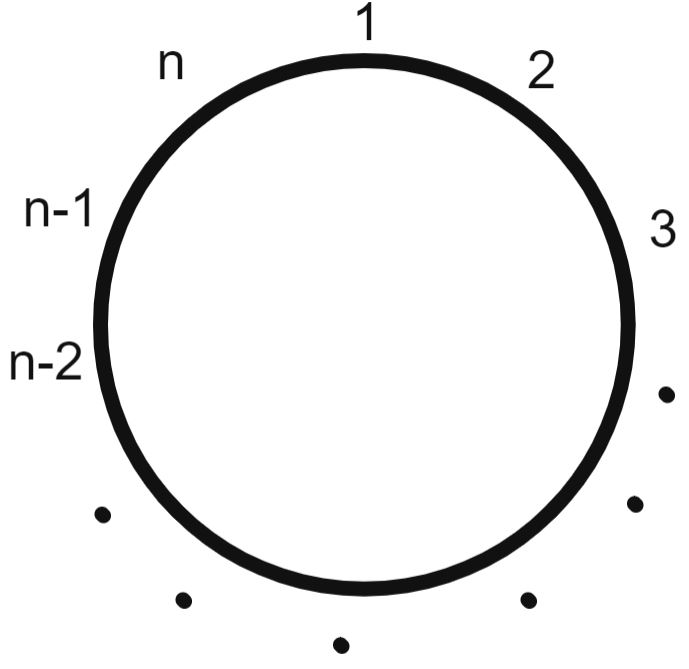
\includegraphics[width=\linewidth]{sol3} %тут поменять имя пикчи
    \end{figure}
    \end{minipage}
\end{minipage}

\textbf{Дефолтные математические знаки и символы:}\\
$\geqslant$,
$\leqslant$,
$a^{b}$,
$x_{i}$,
$\sqrt{a}$,
$\frac{a}{b}$,
$\displaystyle \frac{a}{b}$,
$\cdot$
$\;\Rightarrow\;$,
$\;\Leftrightarrow\;$,
$1{,}2$.
О промежутках:
$a\!b$,
$a\,b$,
$a\:b$,
$a\;b$,
$a\quad b$.

\textbf{Стандартные система и совокупность уравнений / неравенств:}\\
$\left\{
\begin{aligned}
f(x) &= 0 \\
g(x) &= 1
\end{aligned}\right.$

$\left[\begin{aligned}
&\left\{\begin{aligned}
f(x) &\geqslant a \\
g(x) &= b
\end{aligned}\right.\\
&\left\{\begin{aligned}
f(x) &< a \\
g(x) &= -b
\end{aligned}\right.
\end{aligned}\right.$

\subsection*{\textcolor{Emerald}{\textbf{Не математическое, но полезное:}}}
% комментарий в любом месте документа, который нигде не будет видно. Можно использовать для написания заметок-вопросов по задачам
\textbf{Пример таблицы:}

\begin{tabular}{|c|c|c|}
\hline
    $a$ & $b$ & текст
\\\hline
    $c$ & $d$ & мораль
\\\hline
\end{tabular}\\

\textbf{Отступы:} между\smallskip\\ строками\medskip\\ \textbf{Тире} --- это три дефиса.\\
\textbf{Списки:}
\begin{mylist}
\item [$\bullet$] это был пункт а
\item [2)] а это уже пункт номер 2 с изменённым заголовком
\end{mylist}

\subsection*{\textcolor{Emerald}{\textbf{Всё, неупомянутое выше (или если просто что-то не так):}}}
\begin{mylist}
\item [$\bullet$] Решение отдельных вопросов касательно ТеХа нужно искать в \href{https://www.mccme.ru/free-books/llang/newllang.pdf}{Львовском}.

\item [$\bullet$] Найти произвольный символ, который нужен, можно в \href{http://detexify.kirelabs.org/classify.html}{Detexify}.

\item [$\bullet$] Если возникли сомнения при решении, ответ практически ко всем задачам можно проверить с помощью \href{https://www.wolframalpha.com/}{WolframAlpha}.

\item [$\bullet$] Если в задаче нужно создать картинку, то лучше пока отложить эту задачу. Все графики планируется централизованно нарисовать (или перерисовать) в геогебре.

\item [\textcolor{brown}{\textbf{!!}}] Важно ставить \textcolor{red}{\textbf{$\spadesuit$}}
(или просто red) в тело задачи в случае серьёзных вопросов к решению и какой-то вопиющей лажи.

\item [\textcolor{brown}{\textbf{!!}}] Важно ставить \textcolor{olive}{\textbf{$\spadesuit$}}
(или просто olive) в тело задачи в случае не самого удачного текста и кривых отступов.
\end{mylist}

\subsection*{\textcolor{Violet}{\textbf{Комментарии:}}}% а также невидимые комментарии - так можно оставлять заметки-вопросы прямо в задаче, чтобы потом было понятно, в чём вопрос.
\begin{mylist}
\item [$\skull$] Переставлять задачи местами --- очень плохая идея.

\item [$\smiley$] При двойном клике по тексту pdf справа происходит автоматический переход к этому месту в латех-коде, а для обратного перехода можно нажать стрелку вправо (висит сверху между pdf и латех-кодом).

\item [$\smiley$] Если есть размышления, дописывать red/olive к задаче или не дописывать, то лучше всё-таки дописать.

\item [$\skull$] Самое плохое, что можно сделать --- написать в любое поле из трёх (НаписанноеРешение/ВерныйОтвет/Подсказка) только половину того, что надо, никак это не отметить, и потом пойти дальше.\\ Нужно в этот момент писать red/olive в случайном месте задачи, чтобы потом вычислить это с помощью Ctrl+F по всему документу (и это то, что потом будет делаться долго и тщательно)
\end{mylist}

\newpage
\setcounter{num}{583}

\hypertarget{7.4}{{\centering\section*{\bigskip\\\textcolor{Blue}{\hyperlink{start2}{\textcolor{Blue}{7.4}} Квадратный корень и иррациональные числа.}\vspace{-5mm}}}}

\begin{problem}{Рациональные числа-2, периодические десятичные дроби.}{7.4.1}{9I}{(лёгкая)}
{Представить обыкновенную дробь $\frac 17$ в виде бесконечной десятичной дроби.}
{Поделим число $1 = 1{,}(0)$ на 7 в столбик:\\
\vspace{-4mm}\\\begin{minipage}{\linewidth}
    \begin{minipage}{0.25\linewidth}
    $\arraycolsep=0.05em
\begin{array}{rrrrrrr@{\,}r|r}
1{,}&0&0&0&0&0&0&&\,7\,\qquad\qquad\\
\cline{9-9}
0{,}&7&&&&&&&\,0{,}142857...\\
\cline{1-2}
0{,}&3&0&&&&\\
0{,}&2&8&&&&\\
\cline{2-3}
&&2&0&&&\\
&&1&4&&&\\
\cline{3-4}
&&&6&0&&\\
&&&5&6&&\\
\cline{4-5}
&&&&4&0&\\
&&&&3&5&\\
\cline{5-6}
&&&&&5&0\\
&&&&&4&9\\
\cline{6-7}
&&&&&&1
\end{array}$
    \end{minipage}
    \hspace{0.05\linewidth}
    \begin{minipage}{0.67\linewidth}
    Результаты деления в столбик (первые шесть шагов) изображены слева.\bigskip\\ Таким образом, после шести шагов, мы опять приходим к тому же самому~--- делению единицы на 7.\smallskip\\ Это означает, что в дальнейшем цифры в десятичной записи этого числа будут опять те же, в том же самом порядке, то есть $\frac17 = 0{,}142857142857... = 0{,}(142857)$.\medskip\\
    Итого, $\frac17 = 0{,}(142857)$.
    \end{minipage}
\end{minipage}
}
{$\frac17 = 0{,}(142857)$.}{Подели 1 на 7 в столбик и остановись, когда процесс зациклится.}
\end{problem}

\begin{problem}{Рациональные числа-2, периодические десятичные дроби.}{7.4.1}{9I}{(лёгкая)}
{Представить число $2{,}(36)$ в виде неправильной дроби.}
{Пусть $z = 2{,}(36)$. Тогда $100z = 236{,}(36)$. \\Вычислим разность: $100z - z = 99z = 236{,}(36) - 2{,}(36) = 234$.\\ Таким образом, $99z = 234$, откуда $z = \frac{234}{99} = \frac{26}{11}$.}
{$2{,}(36) = \frac{26}{11}$.}{Использовать стандартный приём, домножив число на $10^{\text{длина периода}}$.\\ Осторожно, полученная неправильная дробь может быть сокращена!}
\end{problem}

\begin{problem}{Рациональные числа-2, периодические десятичные дроби.}{7.4.1}{9I}{(лёгкая)}
{Представить число $3{,}(21)$ в виде неправильной дроби.}
{НаписанноеРешение}
{ВерныйОтвет}{Подсказка}
\end{problem}

\begin{problem}{Рациональные числа-2, периодические десятичные дроби.}{7.4.1}{9I}{*}
{Известно, что $x$ равен бесконечной периодической десятичной дроби $0{,}(729)$.\\Найти обыкновенную дробь $\frac pq$, которая равна $x$.}
{$x = 0{,}(729)$, тогда $1000x = 729{,}(729)$. Получаем, что $999x = 729$.\\
Отсюда $x = \frac{729}{999} = \frac{81}{111} = \frac{27}{37}$.}
{Данная обыкновенная дробь $x = \frac pq = \frac{27}{37}$.}{Сокращай дробь до победного конца!}
\end{problem}

\begin{problem}{Рациональные числа-2, периодические десятичные дроби.}{7.4.1}{9I}{*}
{Известно, что $x$ равен бесконечной периодической десятичной дроби $0{,}(1375)$.\\Найти обыкновенную дробь $\frac pq$, которая равна $x$.}
{Используем стандартный приём~--- рассмотрим число со сдвинутой запятой. В нашем случае это число $10000x = 1375{,}(1375)$. Поэтому $10000x - x = 9999x = 1375{,}(1375) - 0{,}(1375) = 1375$, и $x = \frac{1375}{9999}$. C некоторым трудом, но можно убедиться, что данная дробь может быть сокращена на 11: $x = \frac{1375}{9999} = \frac{11 \cdot 125}{11 \cdot 909} = \frac{125}{909}$. Данная дробь уже очевидно является несократимой, так как её числитель делится только на 5, а знаменатель на 5 не делится.}
{Данная обыкновенная дробь $x = \frac pq = \frac{125}{909}$.}{Дробь, что получится в ответе, сократима.}
\end{problem}

\begin{problem}{Рациональные числа-2, периодические десятичные дроби.}{7.4.1}{9I}{(лёгкая)}
{Решить уравнение: $0{,}(246) \cdot x = 41$.}
{Решением уравнения, очевидно, является $x = 41 : 0{,}(246)$.\\ Выясним, на что же нам надо делить: пусть $y = 0{,}(246) \;\Rightarrow\; 1000y = 246{,}(246)$.\\ Тогда $1000y - y = 999y = 246{,}(246) - 0{,}(246) = 246$. Значит, $999 \cdot y = 246$.\\
Следовательно, $y = \frac{246}{999} = \frac{82}{333}$. Находим $x$: $\,x = 41 : \frac{82}{333} = 41 \cdot \frac{333}{82} = \frac{333}{2} = 166{,}5$.}
{Решением уравнения является $x = 166{,}5$.}{Представить $0{,}(246)$ в виде обыкновенной дроби.\\ Напоминаю, полезно домножить на 10 в степени, равной длине периода.}
\end{problem}

\begin{problem}{Понятие квадратного корня, модуль числа.}{7.4.2}{9D}{(лёгкая)}
{Разбей число на простые множители и вычисли $\sqrt{324}$.}
{НаписанноеРешение}
{$\sqrt{324} = 18$.}{Вначале найди все двойки в числе 324, потом тройки, и так далее, до тех пор пока множители не кончатся.}
\end{problem}

\begin{problem}{Понятие квадратного корня, модуль числа.}{7.4.2}{9D}{(лёгкая)}
{Разбей число на простые множители и вычисли $\sqrt{784}$.}
{Разобьём на множители число $784$. Оно делится на 2:\\ $784 = 2 \cdot 392 = 2 \cdot 2 \cdot 196 = 2 \cdot 2 \cdot 2 \cdot 98 = 2 \cdot 2 \cdot 2 \cdot 2 \cdot 49 = 2^4 \cdot 49 = 2^4 \cdot 7^2$.\\ Таким образом, $\sqrt{784} =\sqrt{2^4 \cdot 7^2} = \sqrt{2^4} \cdot \sqrt{7^2} = 2^2 \cdot 7 = 4\cdot 7 = 28$.}
{$\sqrt{784} = 28$.}{Разложи число 784 на простые множители.}
\end{problem}

\begin{problem}{Понятие квадратного корня, модуль числа.}{7.4.2}{9D}{(лёгкая)}
{Разбей число на простые множители и вычисли $\sqrt{576}$.}
{Разложим число 576 на простые множители.\\ $576 = 2 \cdot 288 = 2 \cdot 2 \cdot 144 = 2 \cdot 2 \cdot 2 \cdot 72 = 2 \cdot 2 \cdot 2 \cdot 2 \cdot 36 = 2^4 \cdot 36 = 2^4 \cdot (2\cdot3)^2 = 2^6 \cdot 3^2$.\\ Получаем, что $\sqrt{576} = \sqrt{2^6 \cdot 3^2} = \sqrt{2^6} \cdot \sqrt{3^2} = 2^3 \cdot 3 = 8 \cdot 3 = 24$.

}
{$\sqrt{576} = 24$.}{Разложи число 576 на простые множители.}
\end{problem}

\begin{problem}{Понятие квадратного корня, модуль числа.}{7.4.2}{9D}{(лёгкая)}
{Разбей число на простые множители и вычисли $\sqrt{7056}$.}
{Разложим число 7056 на простые множители.\\ $7056 = 2 \cdot 3528 = 2 \cdot 2 \cdot 1764 = 2 \cdot 2 \cdot 2 \cdot 882 = 2 \cdot 2 \cdot 2 \cdot 2 \cdot 441 = 2^4 \cdot 3 \cdot 147 = 2^4 \cdot 3 \cdot 3 \cdot 49 = 2^4 \cdot 3^2 \cdot 7^2$. Получаем, что $\sqrt{7056} = \sqrt{2^4 \cdot 3^2 \cdot 7^2} = \sqrt{2^4} \cdot \sqrt{3^2} \cdot \sqrt{7^2} = 4 \cdot 3 \cdot 7 = 84$.

}
{$\sqrt{7056} = 84$.}{Вначале найди все двойки в числе 7056, потом тройки, и так далее, до тех пор пока множители не кончатся.}
\end{problem}

\begin{problem}{Понятие квадратного корня, модуль числа.}{7.4.2}{9D}{(лёгкая)}
{Разбей число на простые множители и вычисли $\sqrt{27225}$.}
{Разложим число 27225 на простые множители. Поскольку на 2 оно не делится, начинаем с 3 (выполнен признак делимости на 3, сумма цифр равна 18).
$$27225 = 3 \cdot 9075 = 3 \cdot 3 \cdot 3025 = 3^2 \cdot 5 \cdot 605 = 3^2 \cdot 5 \cdot 5 \cdot 121 = 3^2 \cdot 5^2 \cdot 11^2.$$
Таким образом, $\,\sqrt{27225} = \sqrt{3^2 \cdot 5^2 \cdot 11^2} = \sqrt{3^2} \cdot \sqrt{5^2} \cdot \sqrt{11^2} = 3 \cdot 5 \cdot 11 = 165$.}
{$\sqrt{27225} = 165$.}{Число 27225 делится на 3.}
\end{problem}

\begin{problem}{Понятие квадратного корня, модуль числа.}{7.4.2}{9D}{*}
{Разбей число на простые множители и вычисли $\sqrt{53361}$.}
{Разложим число 53361 на простые множители. Поскольку на 2 оно не делится, начинаем с 3 (выполнен признак делимости на 3, сумма цифр равна 18).\\ $53361 = 3 \cdot 17787 = 3 \cdot 3 \cdot 5929$. Число 5929 на 3 не делится, на 5 тоже, зато делится на 7. Получаем, что $53361 = 3^2 \cdot 7 \cdot 847 = 3^2 \cdot 7 \cdot 7 \cdot 121 = 3^2 \cdot 7^2 \cdot 11^2$.\\ Получаем, что $\sqrt{53361} = \sqrt{3^2 \cdot 7^2 \cdot 11^2} = \sqrt{3^2} \cdot \sqrt{7^2} \cdot \sqrt{11^2} = 3 \cdot 7 \cdot 11 = 231$.}
{$\sqrt{53361} = 231$.}{На 2 подкоренное выражение не делится, поэтому можно начинать с троек, и перебирать простые делители до тех пор, пока множители не кончатся.}
\end{problem}

\begin{problem}{Свойства квадратного корня.}{7.4.3}{9I}{(лёгкая)}
{Вычислить: $(\sqrt{0{,}013} - \sqrt{5{,}2}) : \sqrt{1{,}3}$.}
{Используем одно из свойств деления: $\;(a - b) : c = a : c - b : c$.\\ Получаем, что $(\sqrt{0{,}013} - \sqrt{5{,}2}) : \sqrt{1{,}3} = \sqrt{0{,}013}  : \sqrt{1{,}3} - \sqrt{5{,}2} : \sqrt{1{,}3}$.\\ Теперь используем свойство арифметического корня: $\sqrt{\mathstrut a} : \sqrt{\mathstrut b} = \sqrt{\frac ab} \;\Rightarrow\; $\\
$\sqrt{0{,}013}  : \sqrt{1{,}3} - \sqrt{5{,}2} : \sqrt{1{,}3} = \sqrt{\frac{0{,}013}{1{,}3}} - \sqrt{\frac{5{,}2}{1{,}3}} = \sqrt{\frac{1}{100}} - \sqrt{4} = 0{,}1 - 2 = -1{,}9$.}
{$(\sqrt{0{,}013} - \sqrt{5{,}2}) : \sqrt{1{,}3} = -1{,}9$.}{$(a - b) : c = a : c - b : c$.}
\end{problem}

\begin{problem}{Свойства квадратного корня.}{7.4.3}{9D}{*}
{Существует ли такое натуральное число $n$, большее 1, что значение выражения $\sqrt{n\sqrt{n\sqrt{n}}}$ является натуральным числом?}
{Каждый корень уменьшает вдвое количество множителей у того числа, которое стоит под корнем. Поэтому, нужно придумать какое-то число, множители которого можно <<уполовинить>> три раза подряд. Поскольку $8 : 2 : 2 : 2 = 1$, логично взять число, у которого какой-нибудь делитель присутствует 8 раз.\\ Возьмём число $2 \cdot 2 \cdot 2 \cdot 2 \cdot 2 \cdot 2 \cdot 2 \cdot 2 = 2^8 = 256$. Проверим, что получится:\\
$\sqrt{2^8\sqrt{2^8\sqrt{2^8}}} = \sqrt{2^8\sqrt{2^8 \cdot 2^4}} = \sqrt{2^8\sqrt{2^{12}}} = \sqrt{2^8 \cdot 2^6} = \sqrt{2^{14}} = 2^7 = 128$.\smallskip\\
Получилось натуральное число, такое $n$ существует (и можно догадаться, что оно даже не одно).}
{Существует, например, при $n = 256$ получается 128.\\
\textit{Комментарий}: исходя из основного свойства степени, $a^b \cdot a^c = a^{b+c}$, и определения арифметического корня $\sqrt{n} \cdot \sqrt{n} = n = n^1$, весьма логично определить $n^{\frac12} = \sqrt{n}$.\\ Тогда $\sqrt{n\sqrt{n\sqrt{n}}} = \left(n \cdot \left(n \cdot n^{\frac12}\right)^{\frac12}\right)^{\frac12} = \left(n \cdot \left(n^{\frac32}\right)^{\frac12}\right)^{\frac12} = \left(n \cdot n^{\frac34}\right)^{\frac12} = \left(n^{\frac74}\right)^{\frac12} = n^{\frac78}$, и интуитивно понятно, что $n = p^{8k}$ подойдёт (получим число $p^{8k \cdot \frac78} = p^{7k}$, которое точно будет натуральным). Однако, поскольку дробных степеней у нас ещё не было, строгим доказательством это рассуждение пока не является...}{Допустим, интересующее нас число имеет вид $n = 2^k$.\\ Каждый корень уменьшает показатель степени вдвое, поэтому корень из любого числа в четной степени будет натуральным числом (например, $\sqrt{3^4} = 3^2 = 9$).\\ Что можно сказать о степени, если надо взять 3 корня подряд?}
\end{problem}

\begin{problem}{Действительные числа и их сравнение.}{7.4.4}{79I}{(лёгкая)}
{Освободиться от иррациональности в знаменателе и выяснить, что больше: $$\displaystyle \frac{\sqrt{2}}{\sqrt{5} - \sqrt{2}} \,\text{ или } \,2.$$

}
{НаписанноеРешение}
{ВерныйОтвет}{Подсказка}
\end{problem}

\begin{problem}{Действительные числа и их сравнение.}{7.4.4}{X}{(лёгкая)}
{Избавиться от иррациональности в знаменателе: $\;\displaystyle \frac{3}{\sqrt{7} + \sqrt{2}} = {?}$}
{НаписанноеРешение}
{ВерныйОтвет}{Подсказка}
\end{problem}

\begin{problem}{Действительные числа и их сравнение.}{7.4.4}{9I}{*}
{Найти значение выражения $\sqrt{(5 - 3\sqrt{5})^{2}} - \sqrt{45}$.}
{По определению, $\sqrt{n}$ --- такое положительное число, что $(\sqrt{n})^2 = n$.\\
Как мы можем видеть, в нашем случае подкоренное выражение уже имеет вид $(\ldots)^2$. Однако будем бдительны! Должно получиться положительное число, а в нашем случае $5 - 3\sqrt{5} < 5 - 3\sqrt{4} = 5 - 3\cdot2 = -1 < 0$. Поэтому меняем знак на противоположный, получаем $3\sqrt{5} - 5$, это число уже точно положительно.\\ $\sqrt{45} = \sqrt{5\cdot9} = 3\sqrt{5}$. В итоге имеем $\sqrt{(5 - 3\sqrt{5})^{2}} - \sqrt{45} = 3\sqrt{5} - 5 - 3\sqrt{5} = -5$.}
{$\sqrt{(5 - 3\sqrt{5})^{2}} - \sqrt{45} = -5$.}{В итоге получится целое число. Главное, что нужно не забыть в ходе решения --- после извлечения корня должно получиться неотрицательное число.}
\end{problem}

\begin{problem}{Неравенства и их свойства.}{7.4.5}{6K}{(лёгкая)}
{Петя старше Коли, который старше Миши, Маша старше Коли, а Даша младше Пети, но старше Маши. Кто третий по возрасту?}
{НаписанноеРешение}
{ВерныйОтвет}{Подсказка}
\end{problem}

\begin{problem}{Неравенства и их свойства.}{7.4.5}{6K}{(лёгкая)}
{Какими цифрами можно заменить звёздочки, чтобы получились верные неравенства? Найди все варианты.\smallskip\\ a) $105 \geqslant 7\cdot1{*}$ \hfill b) $234 \leqslant 9\cdot2{*}$ \hfill c) $17\cdot2{*} > 49\star$ \hfill d) $2{*}\cdot1\star < 258$.}
{а) $105 = 7\cdot 15$. Значит, подходит цифра 5, а также все цифры меньше пяти. То есть 0, 1, 2, 3, 4, 5.\\
b) $234 = 9\cdot26$. То есть подходит 6 и любые цифры больше шести: 6, 7, 8, 9.\\
c) $17\cdot29 = 493$. Поэтому цифра на месте первой звёздочки --- однозначно 9.\\ За второй же звёздочкой может быть любая цифра, при которой получится число, меньшее 493, то есть 0, 1, или 2.\vspace{-2mm}\\
d) $\;$ \parbox{7cm}{Самый простой способ решить эту задачу наглядно --- выписать часть таблицы умножения:} $\quad$
\begin{tabular}{|c|c|c|c|c|c|c|c|}
    \hline
    $\times$ & 20 & 21 & 22 & 23 & 24 & 25 & 26 \\
    \hline
    10 & 200 & 210 & 220 & 230 & 240 & 250 & \textcolor{orange}{260} \\
    \hline
    11 & 220 & 231 & 242 & 253 & \textcolor{orange}{264} & ... & ... \\
    \hline
    12 & 240 & 252 & \textcolor{orange}{264} & ... & ... & ... & ... \\
    \hline
    13 & \textcolor{orange}{260} & ... & ... & ... & ... & ... & ... \\
    \hline
\end{tabular}
\smallskip\\ Видно, что всего есть 12 подходящих вариантов.}
{Решения и ответы указаны выше.}{Над с) полезно подумать подольше --- на самом деле подходящих случаев немного. d) можно решить наглядно, выписав часть таблицы умножения.}
\end{problem}

\end{document}